% =============================================================================
%  CHƯƠNG 1 – CƠ SỞ LÝ THUYẾT
% =============================================================================
\chapter{CƠ SỞ LÝ THUYẾT}
\label{ch:chuong1}

Chương này trình bày các nền tảng lý thuyết cần thiết cho việc xây dựng và
giải bài toán phân bổ tài nguyên trong mạng STAR-RIS hỗ trợ RSMA. Trước hết
là tổng quan về yêu cầu của mạng 6G (mục~\ref{sec:6g}). Kế đến là hai công
nghệ chủ chốt: kỹ thuật đa truy nhập RSMA (mục~\ref{sec:rsma}) và bề mặt
phản xạ thông minh STAR-RIS (mục~\ref{sec:starris}). Cuối chương là phần
giới thiệu về học tăng cường sâu (mục~\ref{sec:drl}) và thuật toán MADDPG
với cơ chế CTDE (mục~\ref{sec:maddpg}).

% -----------------------------------------------------------------------------
\section{Tổng quan mạng vô tuyến thế hệ thứ sáu (6G)}
\label{sec:6g}

\subsection{Kiến trúc đa tầng và yêu cầu hệ thống}

Mạng 6G được dự kiến sẽ là một hạ tầng truyền thông toàn diện kết hợp
nhiều tầng vật lý: tầng vũ trụ với các vệ tinh quỹ đạo thấp (LEO) và vệ
tinh địa tĩnh (GEO); tầng không trung với các phương tiện bay không người
lái (UAV), nền tảng độ cao cao (HAPS), STAR-RIS đặt trên thiết bị bay; và
tầng mặt đất với các trạm gốc gNB, trạm nhỏ (small cell), các thiết bị
người dùng và cảm biến IoT \cite{saad2020vision6g}, \cite{tataria20216g}. Hình
\ref{fig:h1_1} minh họa kiến trúc tích hợp đa tầng này, trong đó các tầng
liên kết với nhau qua các đường truyền không dây và hỗ trợ lẫn nhau về
vùng phủ. Sự kết hợp giữa tầng vũ trụ, tầng không trung và tầng mặt đất
giúp mạng 6G đạt được vùng phủ toàn cầu với mật độ kết nối cao và độ tin
cậy cao.

\begin{figure}[t]
  \centering
  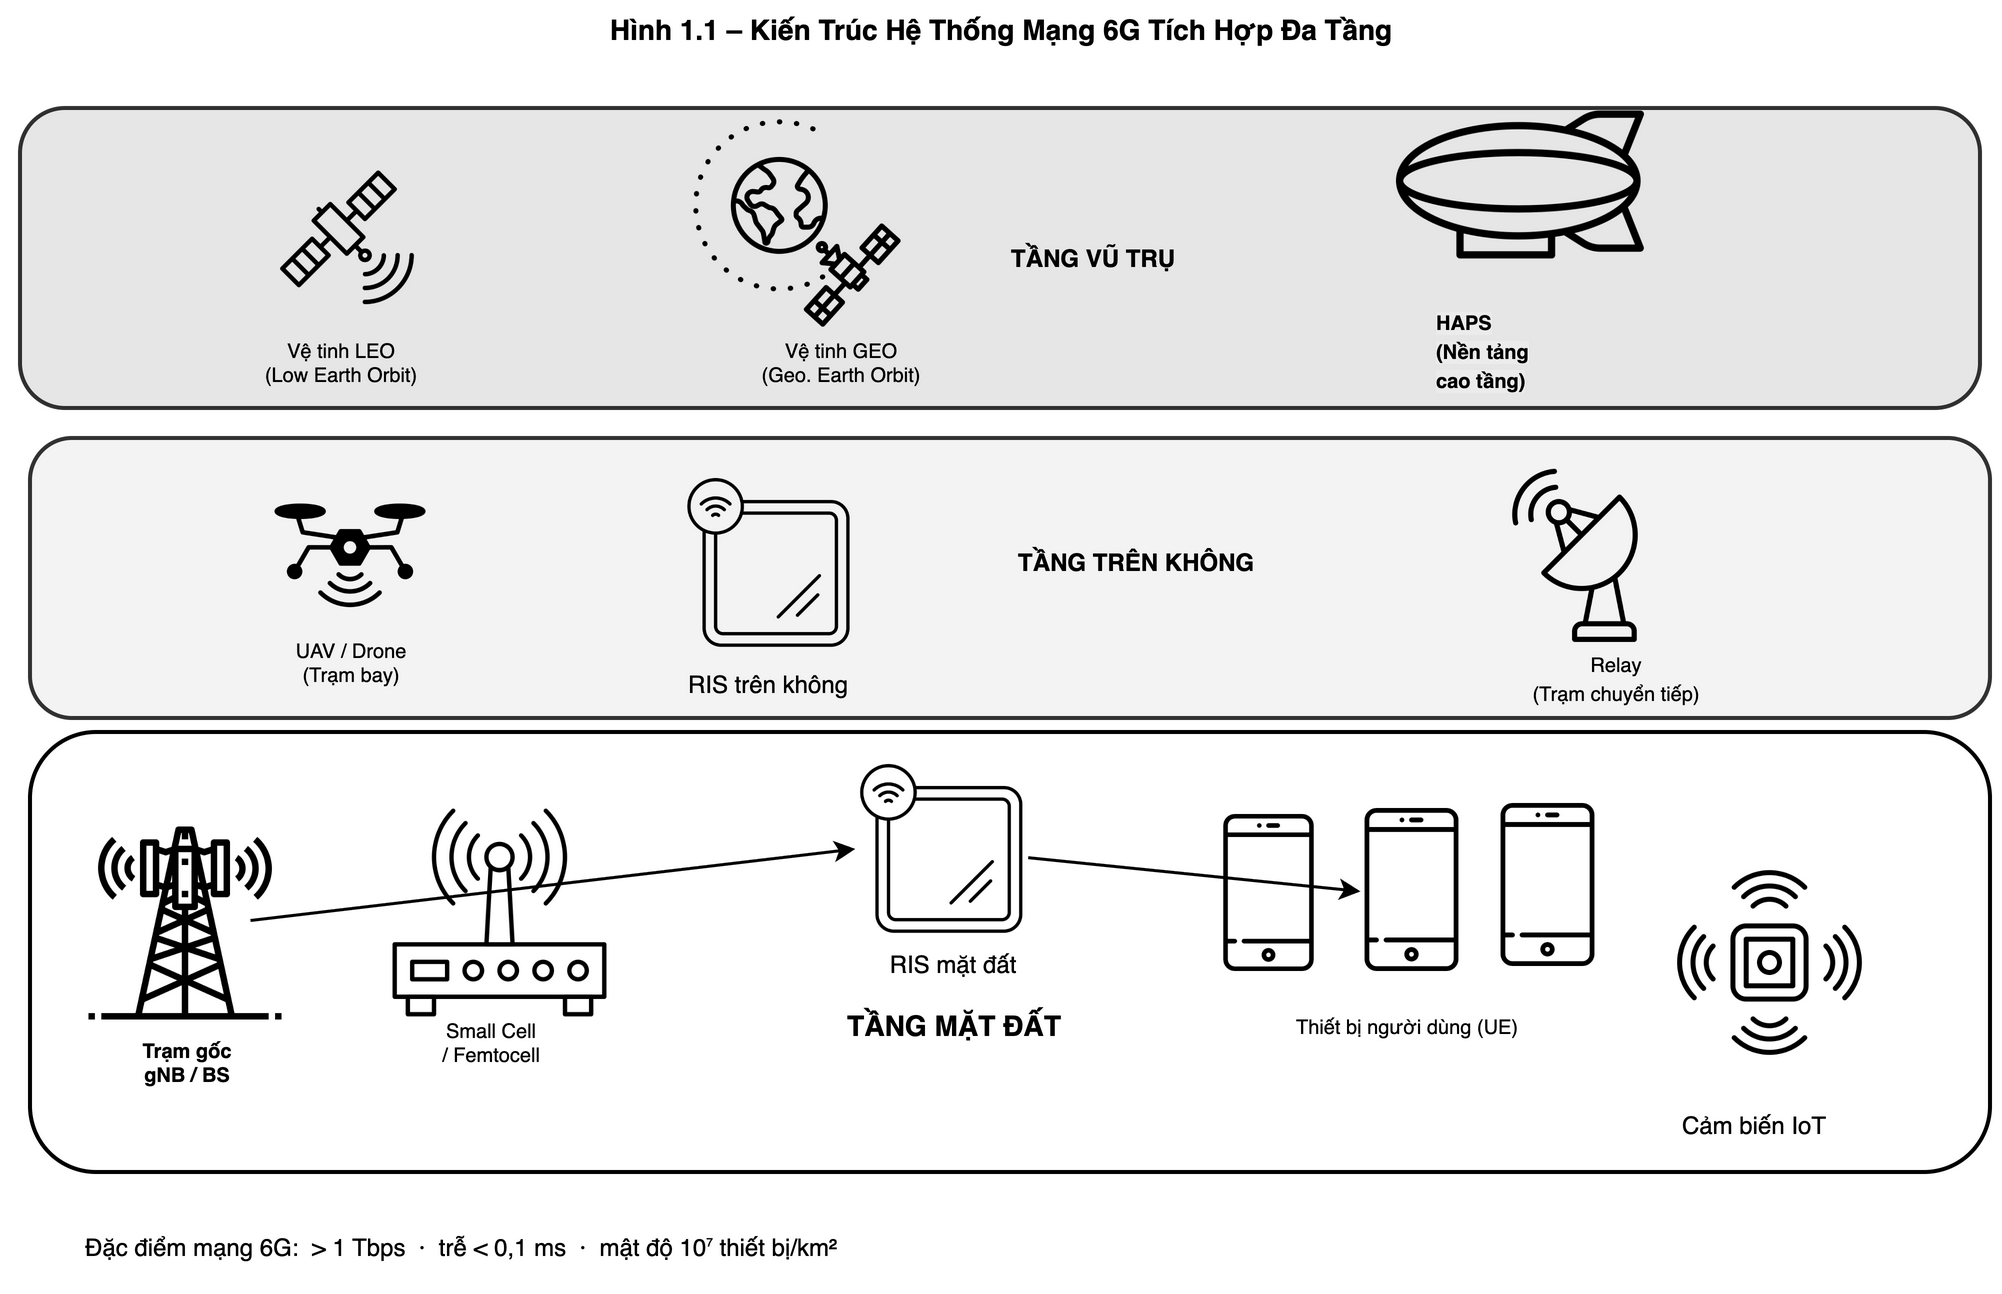
\includegraphics[width=0.92\linewidth]{figures/h1_1_kien_truc_6g.png}
  \caption{Kiến trúc mạng 6G tích hợp đa tầng: vũ trụ, không trung, mặt đất.}
  \label{fig:h1_1}
\end{figure}

So với 5G, các chỉ tiêu của 6G được đặt ra ở mức rất cao
\cite{noor2025aimulti}, \cite{noman2026drl6g}: thông lượng đỉnh trên $1$~Tbps; độ
trễ vô tuyến dưới $100~\mu$s; mật độ kết nối $10^7$ thiết bị/km$^2$; hiệu
quả phổ tăng $10$ lần; hiệu quả năng lượng cải thiện $100$ lần. Để đạt được
các chỉ tiêu này, 6G cần khai thác đồng thời nhiều băng tần (sub-6 GHz,
mmWave, THz), tích hợp trí tuệ nhân tạo ở các tầng vô tuyến và mạng, đồng
thời sử dụng các công nghệ ``điều khiển môi trường truyền sóng''.

\subsection{Thách thức cốt lõi}

Ba thách thức chính cho 6G được nêu trong các báo cáo gần đây
\cite{adams2024rsma}, \cite{priya2024noma}:

\textbf{Khan hiếm phổ tần.} Băng tần dưới 6~GHz đã được khai thác tối đa,
trong khi mmWave và THz tuy có băng thông lớn nhưng chịu suy hao đường
truyền nghiêm trọng và dễ bị che chắn. Cần các kỹ thuật đa truy nhập tiên
tiến vượt qua giới hạn phổ tần.

\textbf{Quản lý nhiễu.} Mật độ kết nối siêu cao ($10^7$ thiết bị/km$^2$)
khiến nhiễu đồng kênh trở thành nút thắt cổ chai. Các kỹ thuật quản lý
nhiễu mềm dẻo (như RSMA) là điều bắt buộc.

\textbf{Hiệu quả năng lượng.} Yêu cầu hiệu quả năng lượng tăng $100$ lần đòi
hỏi các kiến trúc mạng tiêu thụ năng lượng thấp, trong đó RIS thụ động là
một lựa chọn nổi bật \cite{wu2020smart}, \cite{mu2022simultaneously}.

% -----------------------------------------------------------------------------
\section{Kỹ thuật đa truy nhập RSMA}
\label{sec:rsma}

\subsection{Tiến trình phát triển: OMA $\to$ NOMA $\to$ RSMA}

Trong lịch sử các thế hệ vô tuyến, kỹ thuật đa truy nhập đã trải qua nhiều
giai đoạn \cite{mao2022rsma}, \cite{priya2024noma}. Đa truy nhập trực giao
(OMA) như FDMA, TDMA, OFDMA phân bổ tài nguyên (tần số, thời gian, hoặc
sóng mang con) trực giao cho các người dùng. Cách này đảm bảo không có
nhiễu giữa người dùng, nhưng hiệu quả phổ thấp khi số người dùng tăng.
Đa truy nhập không trực giao (NOMA), đặc biệt là NOMA miền công
suất, cho phép nhiều người dùng dùng chung tài nguyên với mức công suất
khác nhau và sử dụng SIC tại phía thu để giải mã liên tiếp. NOMA cải
thiện hiệu quả phổ nhưng nhạy cảm với lỗi pha-đinh, lỗi ước lượng kênh,
và đặc biệt là rất khó tối ưu khi có nhiều người dùng đồng thời cần phục
vụ.

Đa truy nhập theo phân tách tốc độ (RSMA), được Mao và cộng sự
tổng hợp trong \cite{mao2018rsma}, \cite{mao2022rsma}, kết hợp ưu điểm của cả
OMA và NOMA: thông điệp của mỗi người dùng được tách thành phần
chung và phần riêng, truyền chung tài nguyên nhưng với cấu
trúc xử lý hai bậc thay vì xếp tầng tuyến tính như NOMA. Hình \ref{fig:h1_2}
mô tả trực quan sự khác biệt về cách phân bổ tài nguyên giữa OMA, NOMA và
RSMA trong miền tần số/thời gian và công suất. Có thể thấy OMA phân chia
các UE vào các khe tài nguyên trực giao riêng biệt, NOMA chồng các UE
trên cùng tài nguyên với mức công suất khác nhau, còn RSMA bổ sung thêm
một luồng chung được chia sẻ giữa các UE để xử lý nhiễu một cách linh
hoạt hơn.

\begin{figure}[t]
  \centering
  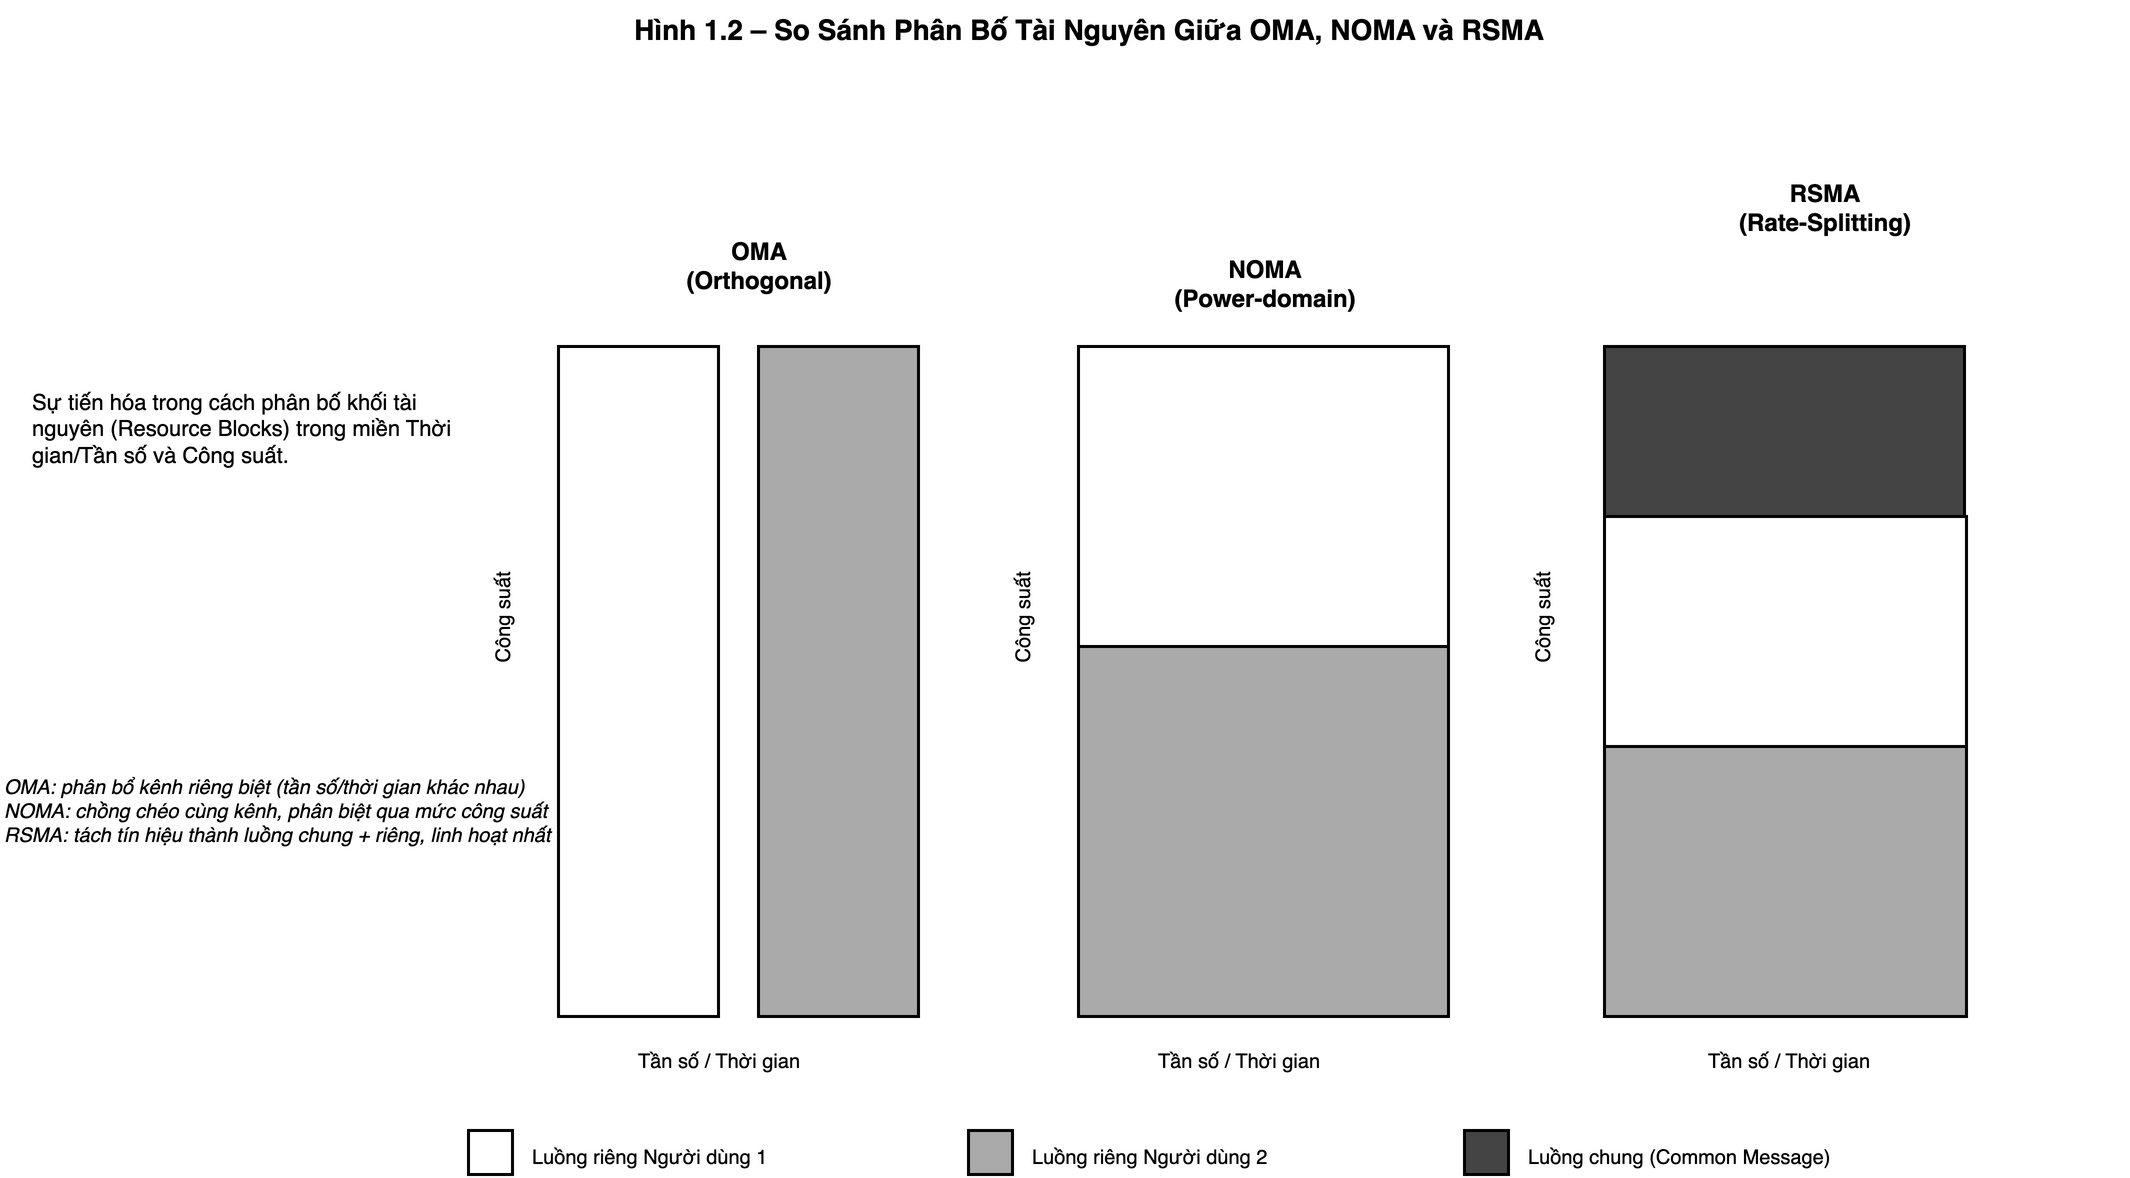
\includegraphics[width=0.95\linewidth]{figures/h1_2_oma_noma_rsma.png}
  \caption{So sánh phân bổ tài nguyên giữa OMA, NOMA và RSMA.}
  \label{fig:h1_2}
\end{figure}

\subsection{Mô hình tín hiệu RSMA lớp đơn}

Xét hệ thống đường xuống một trạm gốc phục vụ $K$ người dùng. Thông điệp
nguyên thủy $W_k$ của người dùng $k$ được tách thành hai phần: phần chung
$W_k^c$ và phần riêng $W_k^p$ \cite{mao2022rsma}, \cite{hua2023learning}. Các
phần chung của tất cả người dùng được kết hợp thành một thông
điệp chung duy nhất $W_c$ rồi mã hóa thành luồng chung $s_c$; các phần
riêng $W_k^p$ được mã hóa độc lập thành các luồng riêng $s_k$. Tín hiệu
phát hợp nhất tại BS có dạng:
\begin{equation}
  x \;=\; \sqrt{P_c}\,s_c \;+\; \sum_{k=1}^{K}\sqrt{P_k}\,s_k,
  \label{eq:rsma_signal}
\end{equation}
trong đó $P_c$ là công suất dành cho luồng chung, $P_k$ là công suất dành
cho luồng riêng của người dùng $k$, với ràng buộc tổng công suất
$P_c + \sum_{k=1}^{K} P_k \le P_{\max}$. Các luồng được chuẩn hóa năng
lượng trung bình đơn vị: $\E\{|s_c|^2\} = \E\{|s_k|^2\} = 1$. Hình
\ref{fig:h1_3} biểu diễn sơ đồ khối xử lý tín hiệu RSMA lớp đơn, gồm bộ
tách thông điệp (Message Splitter), bộ gộp luồng chung (Combiner), bộ mã
hóa và tiền mã hóa (Encoder \& Precoders), khối nhân công suất và bộ
tổng hợp tín hiệu $\Sigma$. Tại phía thu, người dùng giải mã luồng chung
trước, áp dụng khử nhiễu liên tiếp (SIC) và sau đó giải mã luồng riêng
dành riêng cho mình.

\begin{figure}[t]
  \centering
  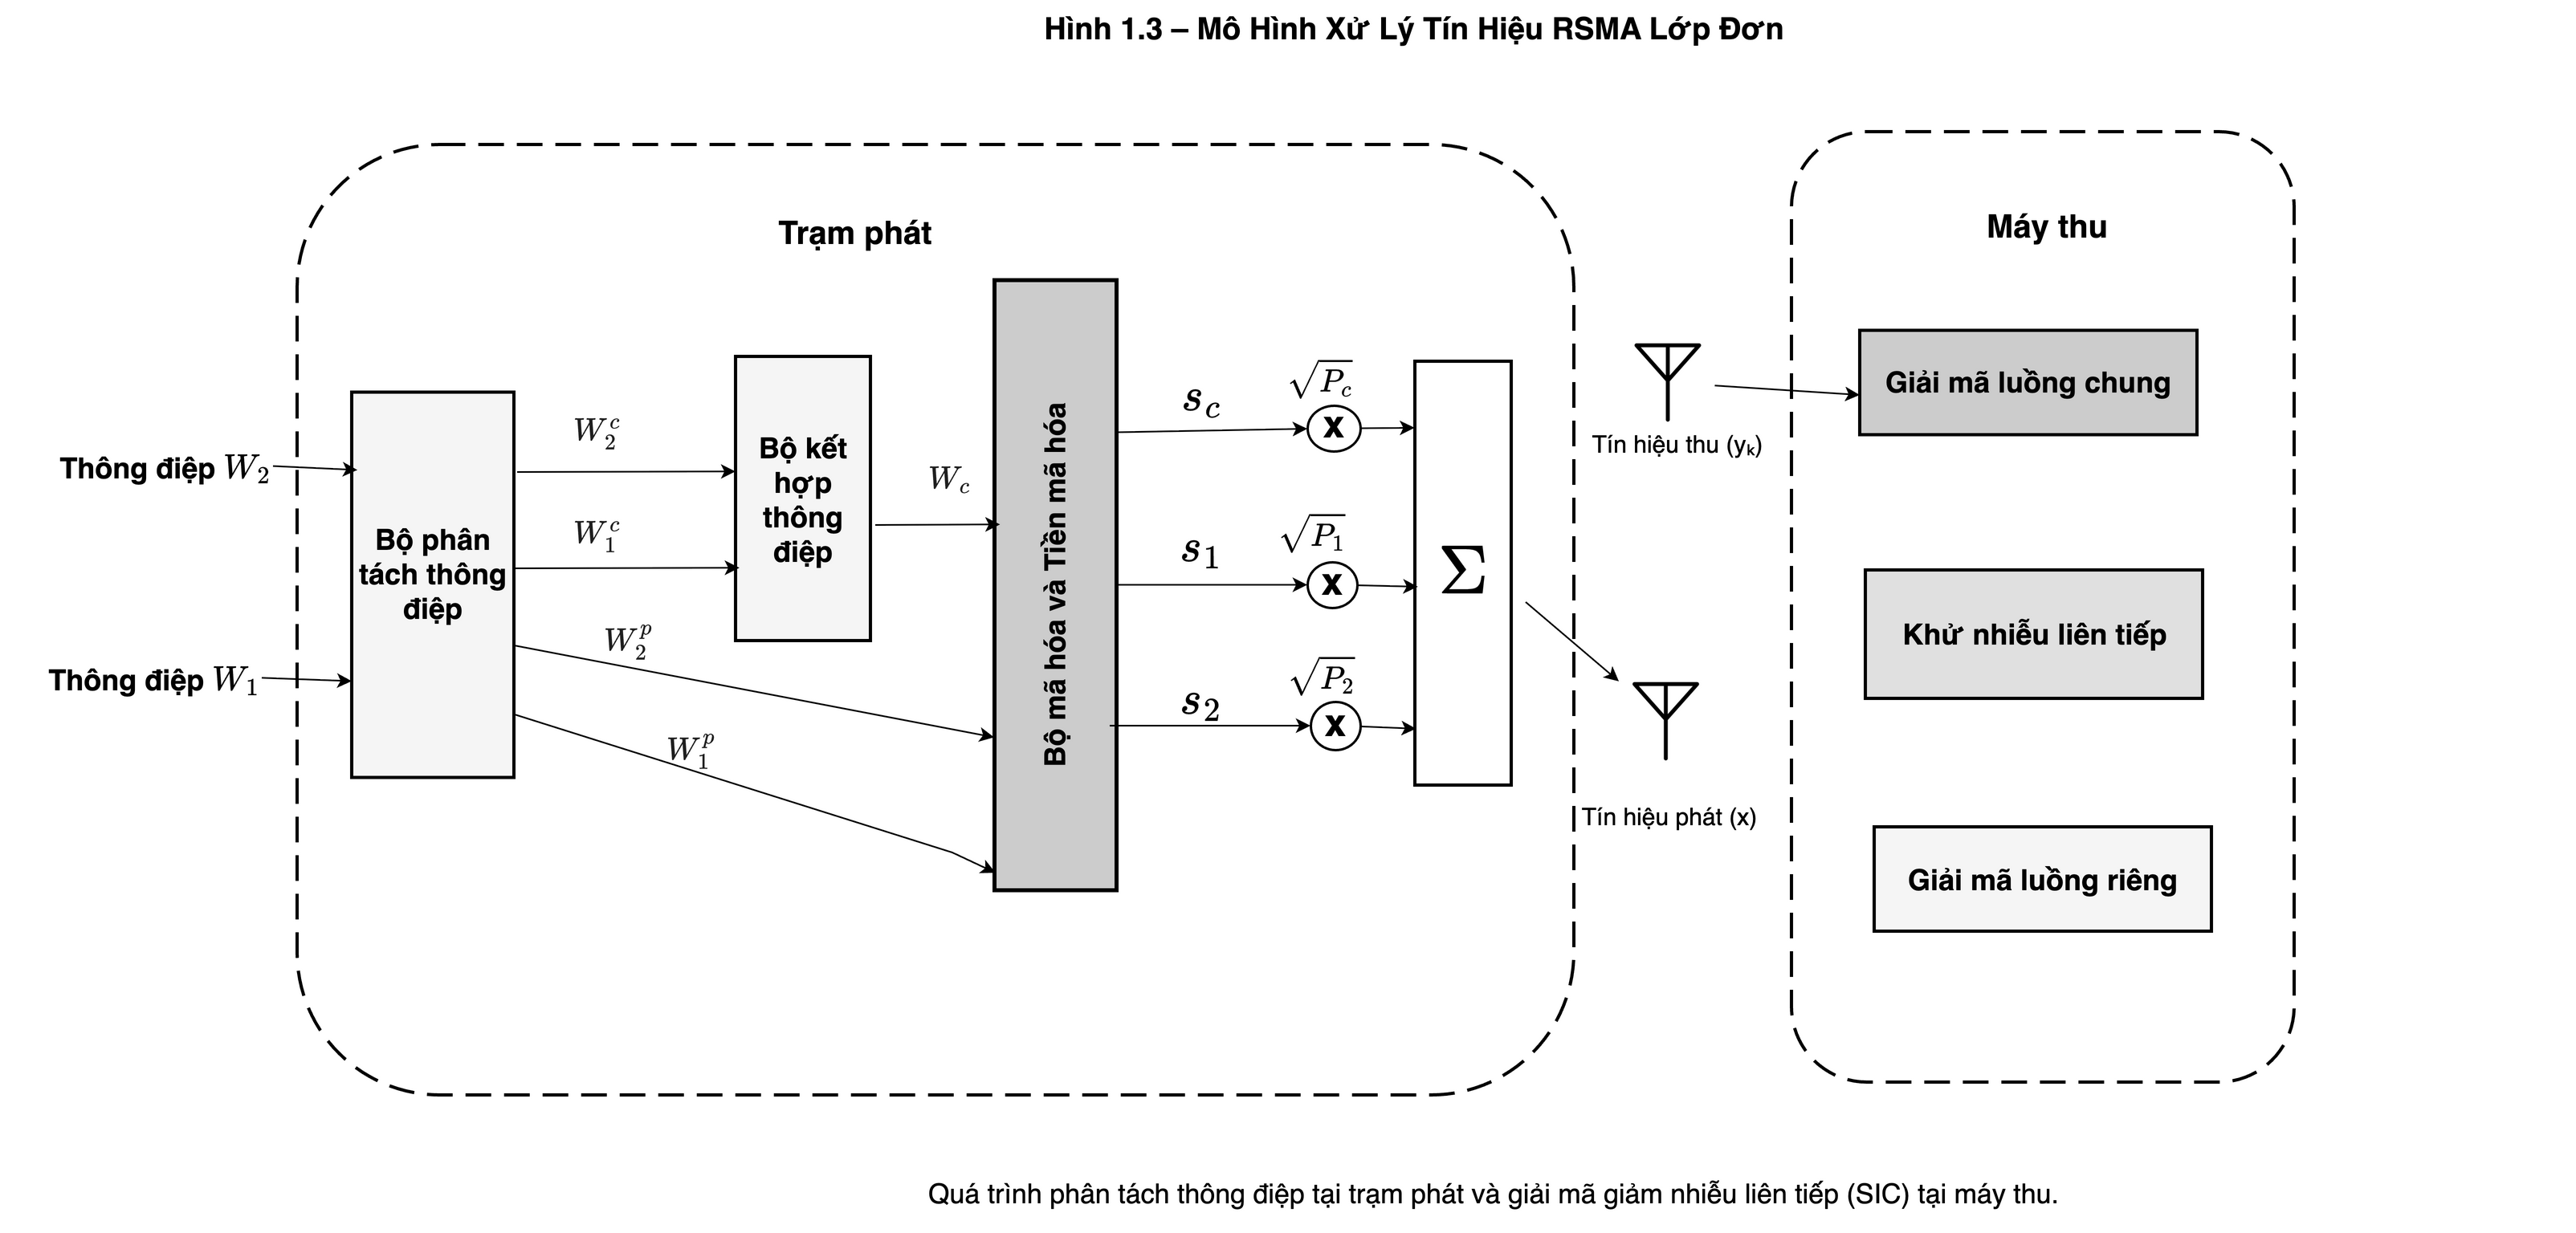
\includegraphics[width=0.95\linewidth]{figures/h1_3_rsma_tin_hieu.png}
  \caption{Sơ đồ khối xử lý tín hiệu RSMA lớp đơn: phía phát (Splitter, Combiner,
  Encoder \& Precoders, $\Sigma$) và phía thu (giải mã luồng chung, SIC, giải mã
  luồng riêng).}
  \label{fig:h1_3}
\end{figure}

Tại phía thu, người dùng $k$ nhận được tín hiệu $y_k$ qua kênh hiệu dụng
$h_{eff,k}$ (sẽ trình bày chi tiết ở chương sau). Quá trình giải mã gồm
hai bước:
\begin{enumerate}[label=(\arabic*),leftmargin=*]
\item Giải mã luồng chung $\hat s_c$, xem các luồng riêng là nhiễu.
\item Áp dụng SIC để trừ ảnh hưởng của $\hat s_c$, sau đó giải mã luồng
riêng $\hat s_k$ dành cho mình, xem các luồng riêng còn lại là nhiễu.
\end{enumerate}

Tốc độ luồng chung của người dùng $k$ là
$R_{c,k} = \log_2(1+\gamma_{c,k})$ với $\gamma_{c,k}$ là SINR luồng chung;
tốc độ luồng riêng là $R_{p,k} = \log_2(1+\gamma_{p,k})$. Vì luồng chung
phải được giải mã thành công bởi mọi người dùng nên tốc độ luồng
chung khả thi bị giới hạn bởi người dùng yếu nhất:
\begin{equation}
  R_c \;=\; \min_{k\in\{1,\ldots,K\}}\, R_{c,k}.
  \label{eq:rc_minmax}
\end{equation}
Tổng tốc độ thu được của người dùng $k$ là
\begin{equation}
  R_k \;=\; c_k\,R_c \;+\; R_{p,k},
  \label{eq:rk}
\end{equation}
trong đó $c_k \in [0,1]$ là tỷ lệ luồng chung phân chia cho người dùng $k$,
thỏa $\sum_{k=1}^K c_k = 1$. Tổng tốc độ toàn hệ thống được định nghĩa là
$R_{\text{sum}} = \sum_{k=1}^{K} R_k$.

\subsection{Ưu điểm RSMA trong quản lý nhiễu}

So với OMA và NOMA, RSMA mang lại ba ưu điểm \cite{mao2022rsma}, \cite{priya2024noma}, \cite{irkicatal2024deep}:

\textbf{(i) Quản lý nhiễu mềm dẻo.} Bằng việc điều chỉnh tỷ lệ tách
$\{c_k\}$ và công suất $\{P_c, P_k\}$, RSMA có thể chuyển trạng thái
giữa hai cực: ``coi nhiễu như tín hiệu mong muốn'' (như SDMA) và ``khử
nhiễu hoàn toàn'' (như NOMA truyền thống). Vì vậy RSMA bao hàm OMA, SDMA
và NOMA như các trường hợp đặc biệt.

\textbf{(ii) Bền vững với lỗi CSI.} RSMA cho phép phía phát đặt một phần
năng lượng vào luồng chung, vốn được giải mã trước khi gặp nhiễu phá
hủy do lỗi CSI, nhờ đó giảm thiểu suy giảm hiệu năng so với NOMA tinh
khiết \cite{wu2024deep}, \cite{cernaloli2023meta}.

\textbf{(iii) Tương thích với SIC một bước.} RSMA chỉ yêu cầu một bước SIC
tại phía thu (giải mã luồng chung trước), đơn giản hơn so với NOMA cần
SIC liên tiếp đối với mỗi cặp người dùng.

% -----------------------------------------------------------------------------
\section{Công nghệ STAR-RIS}
\label{sec:starris}

\subsection{Tổng quan RIS và các giới hạn}

Bề mặt phản xạ thông minh (Reconfigurable Intelligent Surface
RIS) là một mặt phẳng gồm nhiều phần tử thụ động, mỗi phần tử có thể được
điều chỉnh pha (và đôi khi cả biên độ) thông qua các diode PIN hoặc vật
liệu meta. Khi tín hiệu tới mặt phẳng, mỗi phần tử áp dụng một pha dịch
$\phi_n$ trước khi tái phát ra, tạo nên hiệu ứng định dạng tia
``trên không'' mà không cần các bộ khuếch đại RF chủ động
\cite{wu2020smart}. RIS truyền thống chỉ có thể phản xạ tín hiệu, do đó
chỉ phục vụ người dùng nằm trong nửa không gian phía trước RIS
($180^\circ$). Người dùng ở phía sau RIS không nhận được tín hiệu cải
thiện, một hạn chế lớn trong các kịch bản triển khai thực tế.

\subsection{Nguyên lý hoạt động STAR-RIS}

STAR-RIS giải quyết hạn chế trên bằng cách cho phép mỗi phần tử
đồng thời phản xạ một phần năng lượng vào nửa không gian phía
trước (vùng phản xạ R) và truyền qua một phần năng lượng sang nửa không
gian phía sau (vùng truyền qua T), với pha của hai thành phần được điều
chỉnh độc lập \cite{liu2021starris}, \cite{mu2022simultaneously}. Hình
\ref{fig:h1_4} so sánh trực quan vùng phủ của RIS truyền thống với
STAR-RIS, cho thấy STAR-RIS mở rộng vùng phục vụ từ nửa không gian
$180^\circ$ thành toàn không gian $360^\circ$. Điều này đặc biệt có giá
trị trong các kịch bản UE phân bố ở cả hai phía mặt phẳng RIS, như khi
RIS được lắp đặt trên tường tòa nhà hoặc trên thiết bị bay.

\begin{figure}[t]
  \centering
  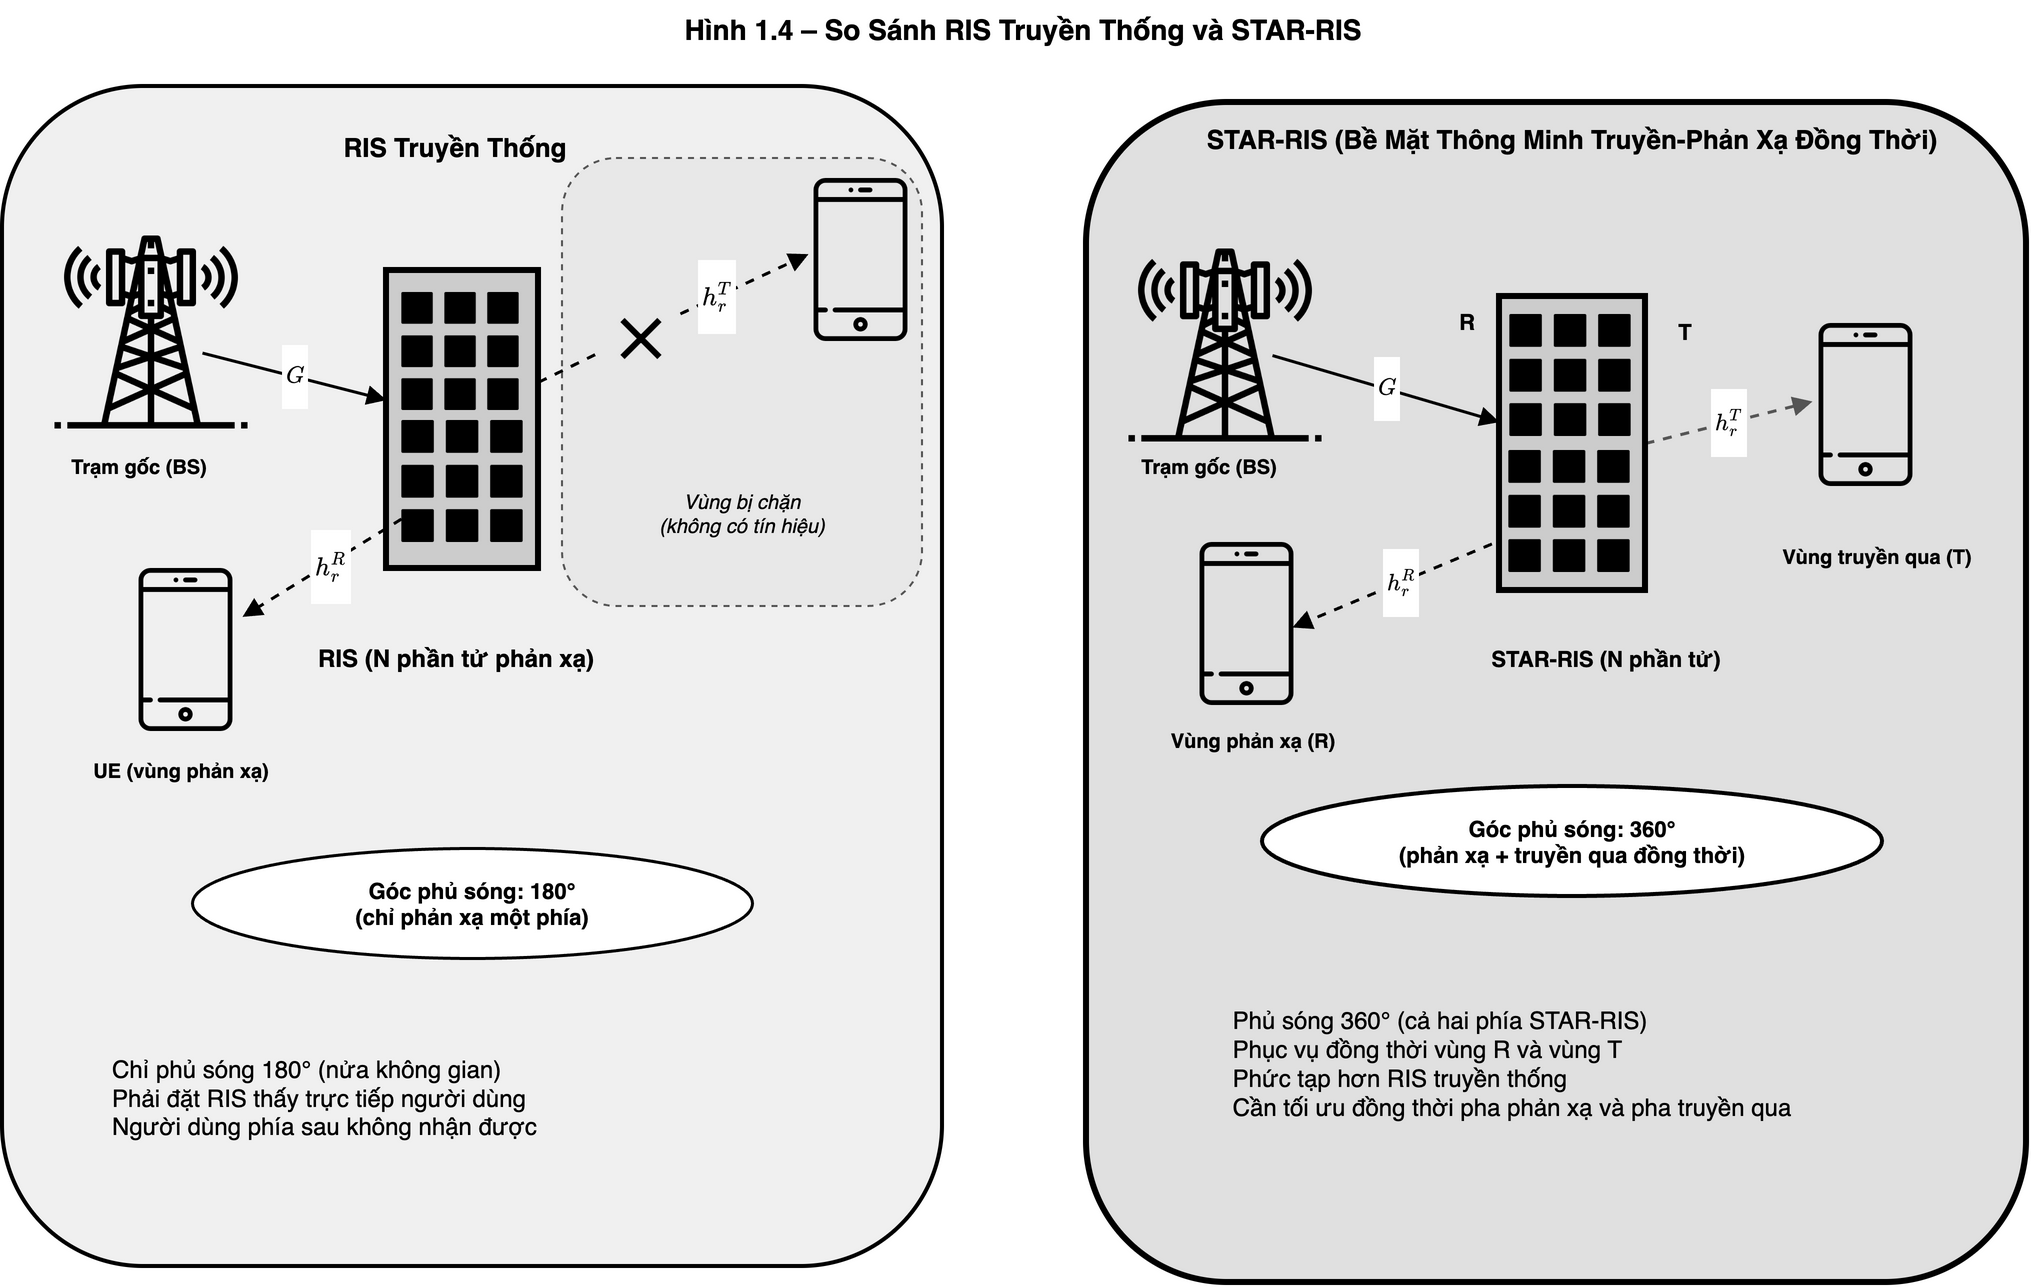
\includegraphics[width=0.92\linewidth]{figures/h1_4_star_ris_vs_ris.png}
  \caption{So sánh vùng phủ sóng: RIS truyền thống ($180^\circ$) và STAR-RIS
  ($360^\circ$). STAR-RIS phục vụ người dùng ở cả hai phía của bề mặt.}
  \label{fig:h1_4}
\end{figure}

Đối với phần tử thứ $n$ của STAR-RIS, hệ số phản xạ và truyền qua được
mô tả bởi các số phức:
\begin{equation}
\Phi_n^R = \sqrt{\beta_n^R}\,e^{j\theta_n^R}, \qquad
\Phi_n^T = \sqrt{\beta_n^T}\,e^{j\theta_n^T},
\label{eq:starris_coef}
\end{equation}
trong đó $\beta_n^R, \beta_n^T \in [0,1]$ là biên độ phản xạ và truyền qua,
$\theta_n^R, \theta_n^T \in [0, 2\pi)$ là pha dịch tương ứng. Bộ điều khiển
STAR-RIS phải điều chỉnh đồng thời $4N$ tham số (hai biên độ và hai pha
cho mỗi phần tử) sao cho cải thiện tổng tốc độ của toàn hệ thống.

\subsection{Ba chế độ vận hành: ES, MS, TS}

STAR-RIS có ba chế độ vận hành cơ bản \cite{mu2022simultaneously}, \cite{liu2021starris}:

\textbf{Chế độ chia sẻ năng lượng (Energy Splitting, ES).} Mỗi phần tử
chia năng lượng tín hiệu tới thành hai phần với tỉ lệ $\beta_n^R$ và
$\beta_n^T$, ràng buộc bởi định luật bảo toàn năng lượng:
\begin{equation}
\beta_n^R + \beta_n^T = 1, \quad \forall n \in \{1,\ldots,N\}.
\label{eq:es_constraint}
\end{equation}
ES là chế độ tổng quát nhất, cho phép STAR-RIS phục vụ đồng thời cả hai
vùng. Đây cũng là chế độ được sử dụng trong Luận văn.

\textbf{Chế độ chuyển đổi chế độ (Mode Switching, MS).} Mỗi phần tử
hoạt động ở một trong hai trạng thái nhị phân: phản xạ thuần
($\beta_n^R = 1, \beta_n^T = 0$) hoặc truyền qua thuần. Mặc dù đơn giản
về phần cứng nhưng MS không khai thác hết khả năng của STAR-RIS.

\textbf{Chế độ chuyển đổi thời gian (Time Switching, TS).} Bề mặt
chuyển toàn bộ phần tử giữa phản xạ và truyền qua theo các khe thời gian,
phù hợp khi yêu cầu phục vụ hai vùng không cần đồng thời.

\subsection{Ứng dụng STAR-RIS trong mạng 6G}

Trong những năm gần đây, STAR-RIS đã được ứng dụng vào nhiều kịch bản 6G:
truyền thông an toàn \cite{kamal2024optimizing}, \cite{zhang2024starrismatrans}, \cite{yang2024covertambc}, truyền thông UAV \cite{singh2024robust}, \cite{perdana2024adaptive}, \cite{huang2024starrisuav}, \cite{nguyen2025star}, truyền thông tích hợp cảm biến
(ISAC) \cite{jin2024arisrsma}, \cite{to2024fairness}, \cite{adams2024rsma},
URLLC \cite{soleymani2024starris}, SWIPT \cite{amiri2024meta}, và nhiều
ứng dụng khác. Trong số đó, kết hợp STAR-RIS với RSMA đã được chứng minh
là tăng hiệu năng đáng kể cho mạng đường xuống \cite{soleymani2024starris}, \cite{gomes2024performance}, \cite{ibrahim2025cognitive}.

% -----------------------------------------------------------------------------
\section{Phân bổ tài nguyên: phương pháp truyền thống và động lực chuyển sang DRL}
\label{sec:resource_allocation}

\subsection{Các phương pháp tối ưu cổ điển}

Bài toán phân bổ tài nguyên cho mạng RIS-RSMA thường có dạng tối ưu phi
lồi nhiều biến (công suất, pha RIS, hệ số tách luồng). Một số phương pháp
cổ điển được sử dụng \cite{mao2022rsma}, \cite{gomes2024performance}:

\begin{itemize}[leftmargin=*]
\item \textbf{Hạ dần khối tọa độ (BCD):} chia tập biến thành các khối, tối
ưu xen kẽ từng khối khi cố định các khối khác. Hội tụ về điểm dừng cục bộ.
\item \textbf{Nới lỏng nửa xác định (SDR):} chuyển biến pha thành ma trận
hạng một, nới lỏng ràng buộc hạng để bài toán trở nên lồi, sau đó dùng
phép phân rã ngẫu nhiên để truy xuất nghiệm xấp xỉ.
\item \textbf{Lập trình lồi xen kẽ (Alternating Convex Optimization, ACO):}
xen kẽ giải nhiều bài toán con lồi nhỏ.
\end{itemize}

\subsection{Hạn chế của phương pháp truyền thống và động lực DRL}

Các phương pháp trên có chung những hạn chế khi áp dụng vào kịch bản
thực tế \cite{noman2026drl6g}, \cite{hieu2021optimal}, \cite{irkicatal2024deep}:

\textbf{Chi phí tính toán cao.} Mỗi vòng lặp BCD/SDR yêu cầu giải nhiều
bài toán lồi phụ trợ, không khả thi cho cập nhật theo thời gian thực khi
kênh truyền biến thiên ở thang ms.

\textbf{Phụ thuộc vào mô hình kênh tường minh.} Khi mô hình kênh sai
lệch (do hardware impairment, lượng tử hóa pha RIS, lỗi ước lượng kênh),
nghiệm tối ưu hóa truyền thống có thể trở nên rất kém.

\textbf{Khó mở rộng quy mô.} Khi $N$ và $K$ tăng (chẳng hạn $N=256$ phần
tử RIS), độ phức tạp tăng phi tuyến mạnh.

Học tăng cường sâu (DRL) khắc phục các hạn chế trên bằng cách học
chính sách phân bổ tài nguyên từ tương tác với môi trường mô phỏng
\cite{sutton2018reinforcement}, \cite{mnih2015human}, \cite{lillicrap2016continuous}.
Sau khi huấn luyện, suy luận chỉ là một lần chạy tiến của mạng nơ-ron với
độ phức tạp $O(1)$ theo kích thước hệ thống đã cố định trước. DRL cũng
học được đặc trưng quan trọng từ dữ liệu thay vì dựa hoàn toàn vào mô
hình giải tích, do đó bền vững hơn trước nhiễu mô hình
\cite{diamanti2023energy}, \cite{faramarzi2024meta}.

% -----------------------------------------------------------------------------
\section{Học tăng cường sâu (DRL)}
\label{sec:drl}

\subsection{Khung tổng quát của học tăng cường}

Học tăng cường được mô hình hóa dưới dạng quá trình ra quyết định Markov
(MDP), được mô tả bởi bộ năm
$\mathcal{M} = (\mathcal{S}, \mathcal{A}, \mathcal{P}, \mathcal{R}, \gamma)$,
trong đó $\mathcal{S}$ là không gian trạng thái, $\mathcal{A}$ là không
gian hành động, $\mathcal{P}(s_{t+1} | s_t, a_t)$ là hàm chuyển trạng
thái, $\mathcal{R}(s_t, a_t)$ là hàm phần thưởng và $\gamma \in [0,1)$ là
hệ số chiết khấu \cite{sutton2018reinforcement}. Tại mỗi bước thời gian
$t$, tác tử quan sát trạng thái $s_t$, chọn hành động $a_t$ theo chính
sách $\pi(a_t | s_t)$, nhận phần thưởng $r_t$ và chuyển sang trạng thái
mới $s_{t+1}$. Mục tiêu của tác tử là tối đa hóa tổng phần thưởng tích lũy
kỳ vọng:
\begin{equation}
  J(\pi) \;=\; \E_\pi\!\left[\sum_{t=0}^{\infty} \gamma^t r_t\right].
  \label{eq:rl_objective}
\end{equation}
Hình \ref{fig:h1_5} minh họa vòng lặp tương tác giữa tác tử và môi trường
theo khung tổng quát của RL. Mũi tên đi ra từ tác tử biểu diễn hành động
$a_t$ được áp dụng vào môi trường, trong khi mũi tên phản hồi từ môi
trường về tác tử mang theo trạng thái mới $s_{t+1}$ và phần thưởng tức
thời $r_{t+1}$.

\begin{figure}[t]
  \centering
  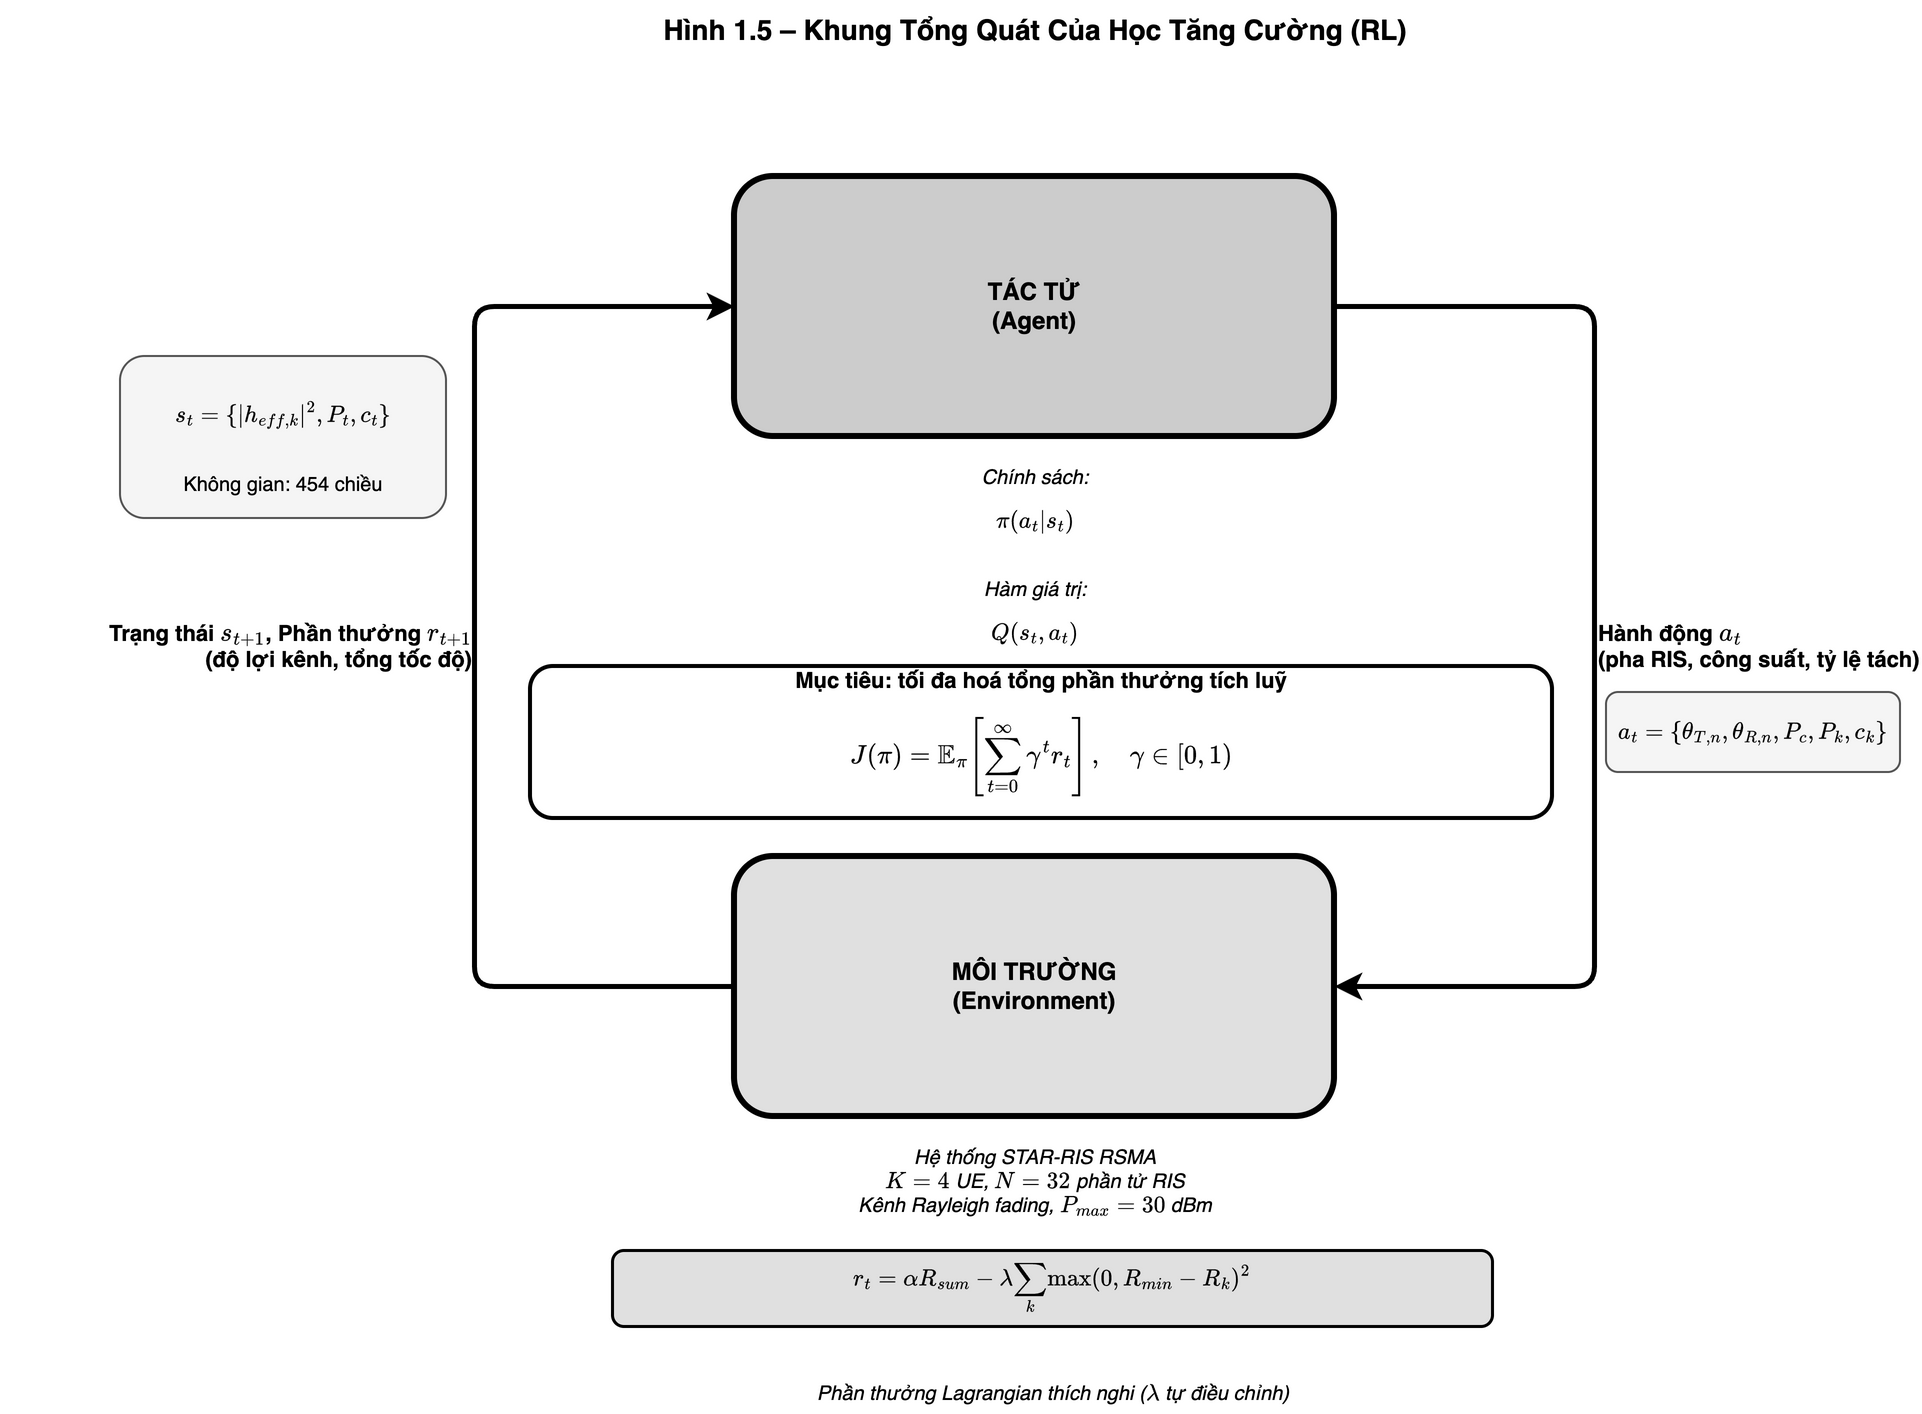
\includegraphics[width=0.78\linewidth]{figures/h1_5_vong_lap_rl.png}
  \caption{Vòng lặp tương tác trong học tăng cường: tác tử quan sát trạng thái,
  chọn hành động, môi trường phản hồi trạng thái mới và phần thưởng.}
  \label{fig:h1_5}
\end{figure}

\subsection{Từ Q-learning đến DQN}

Một trong những thuật toán RL kinh điển nhất là Q-learning, ước lượng
hàm giá trị hành động $Q(s,a)$, là kỳ vọng tổng phần thưởng tích lũy
khi bắt đầu từ trạng thái $s$ và chọn hành động $a$, thông qua phương
trình Bellman:
\begin{equation}
\begin{aligned}
  Q(s,a) \;\leftarrow\;& Q(s,a) \\
  & + \alpha\,\big[\,r + \gamma \max_{a'} Q(s',a') - Q(s,a)\,\big].
\end{aligned}
\end{equation}
Khi không gian trạng thái lớn, Q-learning bảng không khả thi. Mnih và cộng
sự \cite{mnih2015human} đề xuất Deep Q-Network (DQN) sử dụng mạng nơ-ron
sâu để xấp xỉ $Q(s,a)$, mở ra kỷ nguyên DRL. DQN giải quyết được nhiều
bài toán game Atari với mức độ ngang ngửa con người. Tuy nhiên, DQN chỉ
phù hợp với không gian hành động rời rạc.

\subsection{Phương pháp Actor-Critic và DDPG}

Đối với không gian hành động liên tục (như công suất phát, pha RIS),
phương pháp Actor-Critic là lựa chọn tự nhiên. Trong Actor-Critic, có hai
mạng nơ-ron riêng biệt: Actor $\mu_\theta(s)$ học chính sách trực
tiếp, còn Critic $Q_\phi(s,a)$ học hàm giá trị để dẫn dắt huấn
luyện Actor.

Deep Deterministic Policy Gradient (DDPG) \cite{lillicrap2016continuous}
là phiên bản off-policy của Actor-Critic dành cho hành động liên tục, kết
hợp ý tưởng của DQN (replay buffer + target network) với chính sách tất
định. DDPG được cập nhật như sau:
\begin{align}
  \mathcal{L}_{\text{critic}}(\phi) &= \E\big[(Q_\phi(s,a) - y)^2\big],
  \quad y = r + \gamma\,Q_{\phi'}(s', \mu_{\theta'}(s')), \\
  \nabla_\theta J &= \E\big[\nabla_a Q_\phi(s,a)|_{a=\mu_\theta(s)}\,
  \nabla_\theta \mu_\theta(s)\big].
\end{align}
Cập nhật mềm cho mạng mục tiêu:
$\theta' \leftarrow \tau\theta + (1-\tau)\theta'$ với $\tau \ll 1$.

Cải tiến của DDPG bao gồm Twin Delayed DDPG (TD3)
\cite{fujimoto2018addressing} với hai Critic và trì hoãn cập nhật Actor để
giảm sai số overestimation, và Proximal Policy Optimisation (PPO)
\cite{schulman2017proximal} với cập nhật on-policy bị giới hạn để tăng
tính ổn định.

% -----------------------------------------------------------------------------
\section{Thuật toán MADDPG}
\label{sec:maddpg}

\subsection{Bài toán RL đa tác tử}

Khi hệ thống cần được điều khiển bởi nhiều tác tử (ví dụ: BS, STAR-RIS-R,
STAR-RIS-T), bài toán trở thành RL đa tác tử (MARL). Khi áp dụng DDPG
trực tiếp cho từng tác tử (decentralized DDPG), môi trường nhìn từ một
tác tử trở nên không ổn định (non-stationary) vì các tác tử khác
cũng đang thay đổi chính sách. Điều này phá vỡ giả định Markov cố định
và dẫn đến hội tụ kém \cite{lowe2017multi}, \cite{dange2026collaborative}.

\subsection{Cơ chế CTDE trong MADDPG}

Multi-Agent DDPG (MADDPG) đề xuất bởi Lowe và cộng sự
\cite{lowe2017multi} giải quyết vấn đề không ổn định bằng cơ chế
Centralised Training, Decentralised Execution (CTDE):

\textbf{Giai đoạn huấn luyện tập trung.} Mỗi tác tử $i$ có một
Actor $\mu_i$ chỉ thấy quan sát cục bộ $o_i$, nhưng có một
Critic $Q_i$ tập trung thấy toàn bộ quan sát
$\mathbf{o} = (o_1, \ldots, o_N)$ và toàn bộ hành động
$\mathbf{a} = (a_1, \ldots, a_N)$. Vì Critic biết hành động của tất cả
tác tử, môi trường nhìn từ Critic luôn ổn định.

\textbf{Giai đoạn thực thi phân tán.} Sau khi huấn luyện xong, Critic
được bỏ đi; mỗi Actor chỉ cần quan sát cục bộ $o_i$ để sinh ra hành
động $a_i$, không cần thông tin toàn cục. Điều này giúp MADDPG có thể
triển khai trong các kịch bản phân tán thực tế nơi mỗi tác tử chỉ có
quyền truy cập vào thông tin cục bộ. Hình \ref{fig:h1_6} minh họa rõ
hai giai đoạn của cơ chế CTDE, trong đó vùng huấn luyện và vùng thực
thi được tách biệt rõ ràng.

\begin{figure}[t]
  \centering
  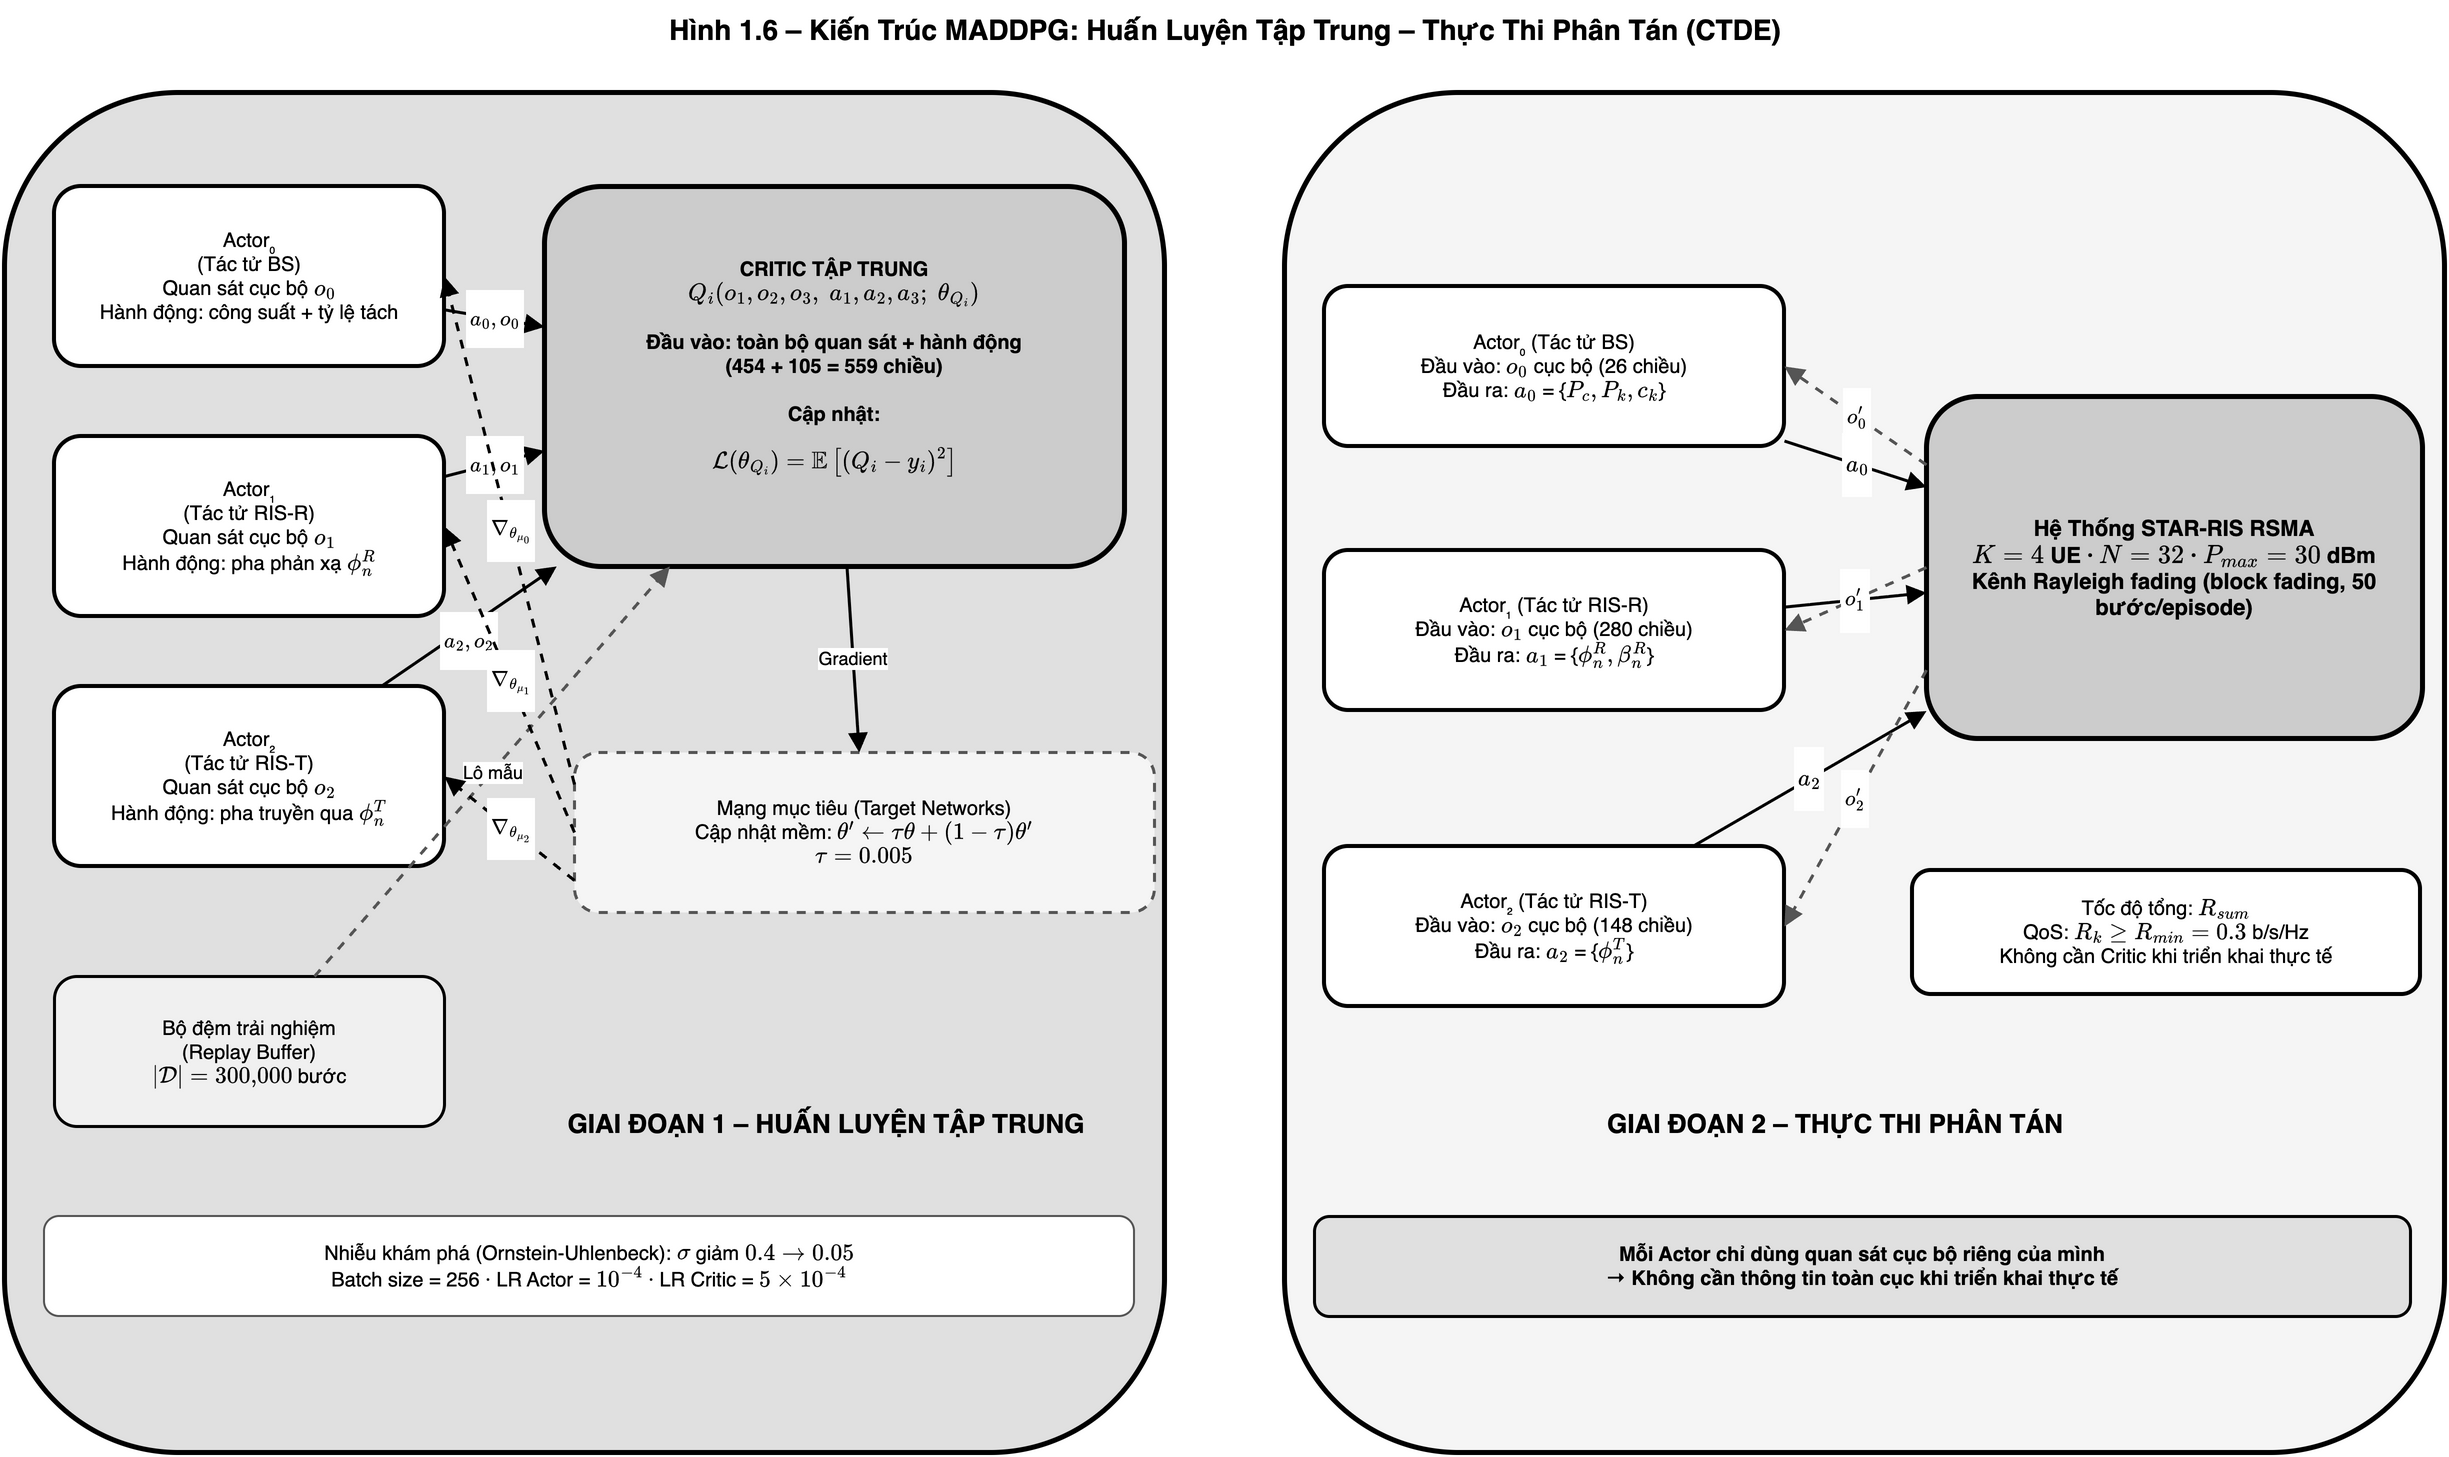
\includegraphics[width=0.95\linewidth]{figures/h1_6_maddpg_ctde.png}
  \caption{Kiến trúc MADDPG với cơ chế CTDE: giai đoạn huấn luyện tập trung
  sử dụng Critic toàn cục, giai đoạn thực thi phân tán chỉ dùng các Actor
  với quan sát cục bộ.}
  \label{fig:h1_6}
\end{figure}

\subsection{So sánh MADDPG với các thuật toán DRL khác}

Bảng \ref{tab:so_sanh_drl} tóm lược ưu nhược điểm của MADDPG so với các
thuật toán DRL phổ biến trong các ứng dụng phân bổ tài nguyên không dây.
Việc so sánh tập trung vào bốn tiêu chí: số lượng tác tử hỗ trợ, ưu điểm
chính, hạn chế chính, và khả năng áp dụng cho không gian hành động liên
tục.

\begin{table}[t]
\centering
\caption{So sánh MADDPG với các thuật toán DRL khác trong phân bổ tài nguyên.}
\label{tab:so_sanh_drl}
\begin{tabular}{p{2.5cm} p{2cm} p{4cm} p{4.5cm}}
\toprule
\textbf{Thuật toán} & \textbf{Số tác tử} & \textbf{Ưu điểm} & \textbf{Hạn chế} \\
\midrule
DQN \cite{mnih2015human}     & 1 & Đơn giản, hội tụ tốt cho hành động rời rạc & Không hỗ trợ hành động liên tục \\
DDPG \cite{lillicrap2016continuous} & 1 & Hành động liên tục, off-policy & Không ổn định khi nhiều tác tử \\
TD3 \cite{fujimoto2018addressing}   & 1 & Khắc phục overestimation của DDPG & Vẫn là đơn tác tử \\
PPO \cite{schulman2017proximal}     & 1 & Cập nhật ổn định, dễ điều chỉnh & On-policy nên kém hiệu quả mẫu \\
\textbf{MADDPG} \cite{lowe2017multi} & $\geq 2$ & CTDE, ổn định trong môi trường đa tác tử & Critic tập trung tăng theo số tác tử \\
\bottomrule
\end{tabular}
\end{table}

MADDPG đã được ứng dụng thành công cho nhiều bài toán không dây gần
đây: phân bổ tài nguyên trong RIS-NOMA \cite{mirza2024multi},
SWIPT-STAR-RIS \cite{dange2026collaborative}, và là cơ sở để Luận
văn này phát triển khuôn khổ phân bổ tài nguyên trong STAR-RIS-RSMA.

% -----------------------------------------------------------------------------
\section{Khoảng trống nghiên cứu và động lực}
\label{sec:research_gap}

Phần này tổng hợp các hạn chế của ba hướng tiếp cận hiện hành đối với
bài toán phân bổ tài nguyên trong mạng STAR-RIS RSMA, từ đó xác định
khoảng trống nghiên cứu (research gap) mà Luận văn hướng tới.

\subsection{Hạn chế của RSMA độc lập}

RSMA độc lập, nghĩa là RSMA không kết hợp với RIS, đã được chứng minh
là vượt trội OMA và NOMA về quản lý nhiễu trong cấu hình MISO/MIMO
\cite{mao2018rsma}, \cite{mao2022rsma}. Tuy nhiên, khi UE nằm trong vùng
NLoS hoặc bị chướng ngại vật che chắn, kênh hiệu dụng suy giảm nghiêm
trọng (xấp xỉ $-25$ dB trong các đánh giá điển hình), khiến luồng chung
$R_c = \min_k R_{c,k}$ bị giới hạn bởi người dùng yếu nhất. Nói cách
khác, RSMA độc lập không cải thiện được điều kiện truyền sóng vật lý
mà chỉ cải thiện việc xử lý nhiễu, do đó hiệu năng vẫn bị giới hạn bởi
kênh truyền cơ sở.

\subsection{Hạn chế của tối ưu STAR-RIS truyền thống}

Các phương pháp tối ưu cổ điển cho STAR-RIS như tối ưu xen kẽ
(Alternating Optimization, AO), hạ dần khối tọa độ (Block Coordinate
Descent, BCD) và nới lỏng nửa xác định (Semidefinite Relaxation, SDR)
yêu cầu giải nhiều bài toán lồi phụ trợ trong mỗi vòng lặp
\cite{wu2020smart}, \cite{soleymani2024starris}. Với $N$ phần tử
STAR-RIS, mỗi vòng SDR có độ phức tạp $\mathcal{O}(N^6)$ hoặc cao hơn,
trong khi BCD đặc trưng cần $50$--$100$ vòng lặp để hội tụ. Tổng chi
phí tính toán này không phù hợp với yêu cầu thời gian thực của 6G, nơi
khoảng coherence kênh chỉ kéo dài cỡ vài mili-giây. Hơn nữa, các phương
pháp này yêu cầu hiểu biết tường minh về mô hình kênh và thường phải
được thiết kế lại khi cấu hình hệ thống thay đổi.

\subsection{Hạn chế của DRL đơn tác tử}

DRL đơn tác tử (như DDPG, TD3, PPO) áp dụng cho bài toán P0 đặt toàn
bộ không gian hành động vào một mạng Actor duy nhất. Với $N=32$ và
$K=4$, không gian hành động hợp nhất có $105$ chiều, bao gồm các đại
lượng có ý nghĩa vật lý hoàn toàn khác nhau: công suất phát $\{P_c,
P_k\}$, tỷ lệ phân chia $\{c_k\}$, pha và biên độ STAR-RIS $\{\theta_n^X,
\beta_n^R\}$. Tác tử đơn không khai thác được cấu trúc phân rã tự nhiên
của bài toán, dẫn đến không gian khám phá lớn và độ phức tạp huấn luyện
cao. Kết quả thực nghiệm trong Chương \ref{ch:chuong4} (Bảng
\ref{tab:algorithm_comparison}) sẽ định lượng hệ quả này: DDPG đơn tác
tử chỉ đạt sum-rate $1{,}98$ b/s/Hz so với $3{,}41$ b/s/Hz của khuôn
khổ đa tác tử đề xuất; hơn nữa, thí nghiệm quét theo $N$ cho thấy
khoảng cách giữa tác tử đơn tốt nhất (TD3) và khuôn khổ đa tác tử
tăng dần theo kích thước không gian hành động, đạt $+0{,}83$ b/s/Hz
tại $N=96$.

\subsection{Khoảng trống nghiên cứu xác định}

Tổng hợp ba hạn chế trên, một khoảng trống nghiên cứu rõ rệt được nhận
diện: \emph{thiếu một khuôn khổ tối ưu chung cho mạng STAR-RIS RSMA
đồng thời đáp ứng bốn đặc tính (i) tối ưu tài nguyên đa miền (công suất,
pha, biên độ, tỷ lệ tách), (ii) xử lý ràng buộc QoS từng người dùng qua
một surrogate ràng buộc mềm với cập nhật đối ngẫu, (iii)
tính khả thi thời gian thực, và (iv) suy luận thời gian thực điều kiện
theo CSI tức thời (real-time CSI-conditioned inference) trong mô hình
kênh động Gauss--Markov.} Luận văn này lấp đầy khoảng trống đó bằng cách
đề xuất khuôn khổ MADDPG-CTDE ba tác tử chuyên dụng. Việc lựa chọn
MADDPG được biện minh từ ba góc độ: cơ chế CTDE giải quyết tính không
ổn định của môi trường đa tác tử thường gặp khi áp dụng DDPG độc lập
cho mỗi tác tử \cite{lowe2017multi}; phân rã ba tác tử khớp tự nhiên
với cấu trúc bài toán (BS điều khiển công suất, RIS-R điều khiển pha
phản xạ, RIS-T điều khiển pha truyền qua); không gian hành động được
ghép cặp (coupled) cũng được phản ánh đúng qua phần thưởng chia sẻ
trong khung cooperative MARL.

% -----------------------------------------------------------------------------
\section{So sánh với các công trình liên quan}
\label{sec:related_work}

Bảng \ref{tab:related_work} so sánh Luận văn này với các công trình
gần đây trên bảy phương diện chủ yếu. Mỗi cột tương ứng với một đặc
tính kỹ thuật quan trọng, từ đó cho phép định vị rõ ràng đóng góp của
Luận văn so với văn liệu hiện tại.

\begin{table}[t]
\centering
\small
\caption{So sánh Luận văn này với các công trình liên quan.}
\label{tab:related_work}
\setlength{\tabcolsep}{4pt}
\begin{tabular}{lccccccc}
\toprule
\textbf{Công trình} & \textbf{STAR-RIS} & \textbf{RSMA} & \textbf{DRL} & \textbf{Đa tác tử} & \textbf{QoS} & \textbf{Mốc AO} & \textbf{CSI-cond.} \\
                    &                   &                &              & \textbf{(MARL)}     &              &              & \textbf{infer.}  \\
\midrule
\cite{mao2022rsma}        & --- & $\checkmark$ & ---           & ---           & ---           & ---           & ---           \\
\cite{liu2021starris}     & $\checkmark$ & --- & ---           & ---           & ---           & ---           & ---           \\
\cite{hieu2021optimal}    & --- & $\checkmark$ & $\checkmark$ & ---           & ---           & ---           & $\checkmark$ \\
\cite{hua2023learning}    & --- & $\checkmark$ & $\checkmark$ & ---           & ---           & ---           & $\checkmark$ \\
\cite{wu2024deep}         & --- & $\checkmark$ & $\checkmark$ & ---           & ---           & ---           & $\checkmark$ \\
\cite{soleymani2024starris}& $\checkmark$ & $\checkmark$ & --- & ---  & ---           & $\checkmark$ & ---           \\
\cite{gomes2024performance}& $\checkmark$ & $\checkmark$ & --- & ---  & ---           & ---           & ---           \\
\cite{amiri2024meta}      & $\checkmark$ & $\checkmark$ & $\checkmark$ & ---           & ---           & ---           & $\checkmark$ \\
\cite{bao2025heuristic}   & $\checkmark$ & $\checkmark$ & $\checkmark$ & ---           & ---           & ---           & $\checkmark$ \\
\cite{diamanti2023energy} & --- & $\checkmark$ & $\checkmark$ & ---           & $\checkmark$ & ---           & $\checkmark$ \\
\cite{huang2024starrisuav}& $\checkmark$ & --- & $\checkmark$ & ---           & ---           & ---           & $\checkmark$ \\
\cite{dange2026collaborative}& $\checkmark$ & --- & $\checkmark$ & $\checkmark$ & ---           & ---           & $\checkmark$ \\
\cite{faramarzi2024meta}  & $\checkmark$ & $\checkmark$ & $\checkmark$ & ---           & ---           & ---           & $\checkmark$ \\
\midrule
\textbf{Luận văn này}     & $\checkmark$ & $\checkmark$ & $\checkmark$ & $\checkmark$ & $\checkmark$ & $\checkmark$ & $\checkmark$ \\
\bottomrule
\end{tabular}

\vspace{0.2em}
{\footnotesize Ghi chú: $\checkmark$ chỉ ra phương diện được xử lý trong công trình. Cột ``Mốc AO'' biểu thị có sử dụng phương pháp tối ưu xen kẽ (AO/BCD) làm mốc so sánh (không phải cận trên). Cột ``CSI-cond. infer.'' biểu thị khả năng suy luận thời gian thực điều kiện theo CSI tức thời tại thời gian chạy.\par}
\hfill {\footnotesize\itshape Nguồn: Tác giả tổng hợp (2026)}
\end{table}


Quan sát Bảng \ref{tab:related_work} cho thấy phần lớn các công trình
hiện hành chỉ xử lý hai hoặc ba trong bảy phương diện. Các công trình
RSMA cổ điển \cite{mao2022rsma} không xét RIS, trong khi các công trình
RIS-RSMA dùng phương pháp tối ưu cổ điển \cite{soleymani2024starris},
\cite{gomes2024performance} phải giải lại bài toán tối ưu lặp cho từng
thể hiện kênh nên khó đáp ứng thời gian thực. Các
công trình DRL cho RSMA \cite{hieu2021optimal}, \cite{hua2023learning},
\cite{wu2024deep} thường chỉ dùng đơn tác tử và không xét STAR-RIS.
Các công trình STAR-RIS với DRL \cite{huang2024starrisuav},
\cite{dange2026collaborative} chưa kết hợp với RSMA. Đặc biệt, ràng
buộc QoS từng UE và việc dùng một heuristic tối ưu xen kẽ (AO-Grid)
làm mốc so sánh cổ điển là hai đặc tính ít được khảo sát đồng thời
trong các nghiên cứu STAR-RIS RSMA. Luận văn này định vị mình là công
trình kết hợp cả bảy phương diện trong một khuôn khổ thống nhất, đặc
biệt với cơ chế phần thưởng Lagrangian surrogate có các hệ số phạt
$\lambda_k$ per-user cập nhật bằng projected dual gradient.

% -----------------------------------------------------------------------------
\section*{Kết luận chương}
\addcontentsline{toc}{section}{Kết luận chương}

Chương 1 đã cung cấp nền tảng lý thuyết tổng quan cho Luận văn, bao gồm:
yêu cầu khắt khe của 6G; nguyên lý hoạt động của RSMA với mô hình tín hiệu
phân tách thành luồng chung và luồng riêng, sử dụng SIC tại phía thu;
kiến trúc STAR-RIS với ba chế độ vận hành (tập trung vào ES); khuôn khổ
DRL và đặc biệt là thuật toán MADDPG với cơ chế CTDE. Các nội dung này là
cơ sở để Chương 2 xây dựng mô hình hệ thống và phát biểu bài toán tối ưu
P0, đồng thời là tiền đề cho Chương 3 thiết kế khuôn khổ MADDPG đề xuất.
